%%%%%%%%%%%%%%%%%%%%%%%%%%%%%%%%%%%%%%%%%%%%%%%%%%%%%%%
% Please note that whilst this template provides a
% preview of the typeset manuscript for submission, it
% will not necessarily be the final publication layout.
%
% letterpaper/a4paper: US/UK paper size toggle
% num-refs/alpha-refs: numeric/author-year citation and bibliography toggle

%\documentclass[letterpaper]{oup-contemporary}
\documentclass[a4paper,num-refs]{oup-contemporary}

%%% Journal toggle; only specific options recognised.
%%% (Only "gigascience" and "general" are implemented now. Support for other journals is planned.)
\journal{gigascience}

\usepackage{graphicx}
\usepackage{siunitx}

% Additional packages used for code formatting
\usepackage{minted}
\usepackage{tcolorbox}
\usepackage{etoolbox}

% Additional packages for data model figure
\usepackage{forest}
\usepackage{tikz}
\usetikzlibrary{quotes,arrows.meta,3d}

% Local definitions to systematise tool naming
\newcommand{\sgapi}[1]{\texttt{#1}}
\newcommand{\toolname}[1]{\texttt{#1}}
\newcommand{\sgkit}{\texttt{sgkit}}


%%% Flushend: You can add this package to automatically balance the final page, but if things go awry (e.g. section contents appearing out-of-order or entire blocks or paragraphs are coloured), remove it!
% \usepackage{flushend}

% Macros etc for data model figure
% TODO: simplify this code
% flexible cuboid from
% https://tex.stackexchange.com/questions/267982/tikz-easy-drawing-of-cuboids
\makeatletter
\def\tikz@lib@cuboid@get#1{\pgfkeysvalueof{/tikz/cuboid/#1}}
\def\tikz@lib@cuboid@setup{%
	\pgfmathsetlengthmacro{\vxx}%
	{\tikz@lib@cuboid@get{xscale}*cos(\tikz@lib@cuboid@get{xangle})*1cm}
	\pgfmathsetlengthmacro{\vxy}%
	{\tikz@lib@cuboid@get{xscale}*sin(\tikz@lib@cuboid@get{xangle})*1cm}
	\pgfmathsetlengthmacro{\vyx}%
	{\tikz@lib@cuboid@get{yscale}*cos(\tikz@lib@cuboid@get{yangle})*1cm}
	\pgfmathsetlengthmacro{\vyy}%
	{\tikz@lib@cuboid@get{yscale}*sin(\tikz@lib@cuboid@get{yangle})*1cm}
	\pgfmathsetlengthmacro{\vzx}%
	{\tikz@lib@cuboid@get{zscale}*cos(\tikz@lib@cuboid@get{zangle})*1cm}
	\pgfmathsetlengthmacro{\vzy}%
	{\tikz@lib@cuboid@get{zscale}*sin(\tikz@lib@cuboid@get{zangle})*1cm}
}

\def\tikz@lib@cuboid@draw#1--#2--#3\pgf@stop{%
	\begin{scope}[join=bevel,x={(\vxx,\vxy)},y={(\vyx,\vyy)},z={(\vzx,\vzy)}]
		% first fill the faces with global and individual style
		% then draw the grids
		\begin{scope}[canvas is yz plane at x=#1]
			\draw[cuboid/all faces,cuboid/edges,cuboid/right face] 
			(0,0) -- ++(#2,0) -- ++(0,-#3) -- ++(-#2,0) -- cycle;
			\draw[cuboid/all grids,cuboid/right grid] (0,0) grid (#2,-#3);
		\end{scope}
		\begin{scope}[canvas is xy plane at z=0]
			\draw[cuboid/all faces,cuboid/edges,cuboid/front face] 
			(0,0) -- ++(#1,0) --  ++(0,#2) -- ++(-#1,0) -- cycle;
			\draw[cuboid/all grids,cuboid/front grid] (0,0) grid (#1,#2);
		\end{scope}
		\begin{scope}[canvas is xz plane at y=#2]
			\draw[cuboid/all faces,cuboid/edges,cuboid/top face] 
			(0,0) -- ++(#1,0) --  ++(0,-#3) -- ++(-#1,0) -- cycle;
			\draw[cuboid/all grids,cuboid/top grid] (0,0) grid (#1,-#3);
		\end{scope}
		% now, draw the hidden edges
		\draw[cuboid/hidden edges] (0,#2,-#3) -- (0,0,-#3) -- (0,0,0) 
		(0,0,-#3) -- ++(#1,0,0);
		% finally, draw the visible edges 
		\begin{scope}[canvas is yz plane at x=#1]
			\draw[cuboid/all faces,cuboid/right face,cuboid/edges,fill opacity=0] 
			(0,0) -- ++(#2,0) -- ++(0,-#3) -- ++(-#2,0) -- cycle;
		\end{scope}
		\begin{scope}[canvas is xy plane at z=0]
			\draw[cuboid/all faces,cuboid/front face,cuboid/edges,fill opacity=0] 
			(0,0) -- ++(#1,0) --  ++(0,#2) -- ++(-#1,0) -- cycle;
		\end{scope}
		\begin{scope}[canvas is xz plane at y=#2]
			\draw[cuboid/all faces,cuboid/top face,cuboid/edges,fill opacity=0] 
			(0,0) -- ++(#1,0) --  ++(0,-#3) -- ++(-#1,0) -- cycle;
		\end{scope}
		% define the anchors: 8 vertices
		\path (0,#2,0) coordinate (-left top front)
		coordinate (-left front top)
		coordinate (-top left front)
		coordinate (-top front left)
		coordinate (-front top left)
		coordinate (-front left top);
		\path (0,#2,-#3) coordinate (-left top rear)
		coordinate (-left rear top)
		coordinate (-top left rear)
		coordinate (-top rear left)
		coordinate (-rear top left)
		coordinate (-rear left top);
		\path (0,0,-#3) coordinate (-left bottom rear)
		coordinate (-left rear bottom)
		coordinate (-bottom left rear)
		coordinate (-bottom rear left)
		coordinate (-rear bottom left)
		coordinate (-rear left bottom);
		\path (0,0,0) coordinate (-left bottom front)
		coordinate (-left front bottom)
		coordinate (-bottom left front)
		coordinate (-bottom front left)
		coordinate (-front bottom left)
		coordinate (-front left bottom);
		\path (#1,#2,0) coordinate (-right top front)
		coordinate (-right front top)
		coordinate (-top right front)
		coordinate (-top front right)
		coordinate (-front top right)
		coordinate (-front right top);
		\path (#1,#2,-#3) coordinate (-right top rear)
		coordinate (-right rear top)
		coordinate (-top right rear)
		coordinate (-top rear right)
		coordinate (-rear top right)
		coordinate (-rear right top);
		\path (#1,0,-#3) coordinate (-right bottom rear)
		coordinate (-right rear bottom)
		coordinate (-bottom right rear)
		coordinate (-bottom rear right)
		coordinate (-rear bottom right)
		coordinate (-rear right bottom);
		\path (#1,0,0) coordinate (-right bottom front)
		coordinate (-right front bottom)
		coordinate (-bottom right front)
		coordinate (-bottom front right)
		coordinate (-front bottom right)
		coordinate (-front right bottom);
		% centers of the 6 faces
		\coordinate (-left center) at (0,.5*#2,-.5*#3);
		\coordinate (-right center) at (#1,.5*#2,-.5*#3);
		\coordinate (-top center) at (.5*#1,#2,-.5*#3);
		\coordinate (-bottom center) at (.5*#1,0,-.5*#3);
		\coordinate (-front center) at (.5*#1,.5*#2,0);
		\coordinate (-rear center) at (.5*#1,.5*#2,-#3);
		% center of the cuboid
		\coordinate (-center) at (.5*#1,.5*#2,-.5*#3);
		% centers of the 12 edges
		\path (0,#2,-.5*#3) coordinate (-left top center) 
		coordinate (-top left center);
		\path (.5*#1,#2,-#3) coordinate (-top rear center)
		coordinate (-rear top center);
		\path (#1,#2,-.5*#3) coordinate (-right top center)
		coordinate (-top right center);
		\path (.5*#1,#2,0) coordinate (-top front center)
		coordinate (-front top center);
		\path (0,0,-.5*#3) coordinate (-left bottom center) 
		coordinate (-bottom left center);
		\path (.5*#1,0,-#3) coordinate (-bottom rear center)
		coordinate (-rear bottom center);
		\path (#1,0,-.5*#3) coordinate (-right bottom center)
		coordinate (-bottom right center);
		\path (.5*#1,0,0) coordinate (-bottom front center)
		coordinate (-front bottom center);
		\path (0,.5*#2,0) coordinate (-left front center) 
		coordinate (-front left center);
		\path (0,.5*#2,-#3) coordinate (-left rear center)
		coordinate (-rear left center);
		\path (#1,.5*#2,0) coordinate (-right front center)
		coordinate (-front right center);
		\path (#1,.5*#2,-#3) coordinate (-right rear center)
		coordinate (-rear right center);
	\end{scope}
}

\tikzset{
	pics/cuboid/.style = {
		setup code = \tikz@lib@cuboid@setup,
		background code = \tikz@lib@cuboid@draw#1\pgf@stop
	},
	pics/cuboid/.default={1--1--1},
	cuboid/.is family,
	cuboid,
	all faces/.style={fill=white},
	all grids/.style={draw=none},
	front face/.style={},
	front grid/.style={},
	right face/.style={},
	right grid/.style={},
	top face/.style={},
	top grid/.style={},
	edges/.style={},
	hidden edges/.style={draw=none},
	xangle/.initial=0,
	yangle/.initial=90,
	zangle/.initial=210,
	xscale/.initial=1,
	yscale/.initial=1,
	zscale/.initial=0.5
}

\newcommand{\tikzcuboidreset}{
	\tikzset{cuboid,
		all faces/.style={fill=white},
		all grids/.style={draw=none},
		front face/.style={},
		front grid/.style={},
		right face/.style={},
		right grid/.style={},
		top face/.style={},
		top grid/.style={},
		edges/.style={},
		hidden edges/.style={draw=none},
		xangle=0,
		yangle=90,
		zangle=225,
		xscale=1,
		yscale=1,
		zscale=0.5
	}
}

\newcommand{\tikzcuboidset}{\@ifstar\tikzcuboidset@star\tikzcuboidset@nostar} 
\newcommand{\tikzcuboidset@nostar}[1]{\tikzcuboidreset\tikzset{cuboid,#1}}
\newcommand{\tikzcuboidset@star}[1]{\tikzset{cuboid,#1}}
\makeatother


% tentative
\title{Columnar VCF for Biobank scale datasets using Zarr}

%%% Use the \authfn to add symbols for additional footnotes, if any. 1 is reserved for correspondence emails; then continuing with 2 etc for contributions.
\author[1,\authfn{1},\authfn{2}]{First Author}
\author[2,\authfn{1},\authfn{2}]{Second Author}
\author[2]{Third Author}
\author[2,\authfn{1}]{Fourth Author}

\affil[1]{First Institution}
\affil[2]{Second Institution}

%%% Author Notes
\authnote{\authfn{1}abc@uni.edu; alphbeta@lab.edu}
\authnote{\authfn{2}Contributed equally.}

%%% Paper category
\papercat{Paper}

%%% "Short" author for running page header
\runningauthor{First et al.}

%%% Should only be set by an editor
\jvolume{00}
\jnumber{0}
\jyear{2024}

\begin{document}

\begin{frontmatter}
\maketitle

% The Abstract (250 words maximum) should be structured to
% include the following details:
% \textbf{Background}, the context and purpose of
% the study;
% \textbf{Results}, the main findings;
% \textbf{Conclusions}, brief
% summary and potential implications. Please minimize the use of abbreviations
% and do not cite references in the abstract.
% The Abstract (250 words maximum) should be structured to
% include the following details:
% \textbf{Background}, the context and purpose of % the study;
% \textbf{Results}, the main findings;
% \textbf{Conclusions}, brief summary and potential implications.

%% NOTE: this is much too long currently, but keeping for now so we
% can see which stuff migrates to the intro
\begin{abstract}
\textbf{Background:}
Variant Call Format (VCF) is the standard file format for interchanging
genetic variation data and associated quality control metrics.
It provides a well-defined data model and is central to a large ecosystem
of tools interoperating through this format.
The standard row-based encoding of the VCF data model (either as text
or packed binary) emphasises efficient retrieval of all data for a given
variant, but accessing subsets of the data within rows is inefficient.
Biobank-scale datasets currently available 
consist of hundreds of thousands of whole genomes with tens of terabytes
of compressed VCF per chromosome.
Row-based data storage is fundamentally unsuited to such datasets
and these large VCFs represent a major computational bottleneck.

\textbf{Results:}
We present the vcfzarr specification, a columnar encoding of the 
VCF data model using Zarr which makes retrieving subsets of the 
data much more efficient. Zarr is a cloud-native format for storing 
multi-dimensional numerical data, widely used in scientific computing.
We show how this format is competitive with specialised methods for 
storing genotype data in terms of compression ratios, and also performs
well on compressing the high-entropy quality-control fields that 
tend to dominate. We show that performing calculations on the genotype
matrix is much more efficient than standard
approaches based on VCF, and is comparable with state-of-the-art methods
using compiled languages. We demonstrate 
the vcfzarr format (and the vcf2zarr conversion utility) 
on the Genomics England dataset of XX,XXX,XXX samples, showing
an overall reduction in storage of XX, and a reduction in processing 
time of common queries of up to XX fold.

\textbf{Conclusions:}
Large row-encoded VCF files are a major bottleneck for current research, and 
processing these files incurs a substantial economic cost.
The vcfzarr specification, building on widely-used, open-source technologies
has the potential to greatly reduce these costs,
and may enable a diverse ecosystem of next-generation tools for analysing 
genetic variation data.
\end{abstract}

\begin{keywords}
Keyword1; keyword 2; keyword 3 (Three to ten keywords representing the main content of the article)
\end{keywords}
\end{frontmatter}

%%% Key points will be printed at top of second page
\begin{keypoints*}
\begin{itemize}
\item This is the first point
\item This is the second point
\item One last point.
\end{itemize}
\end{keypoints*}

\section{Background}
[Four paragraphs. (1) What is VCF, and the good things it has done. 
(2) Explosion in dataset size. Summary of where we're at in terms of biobanks
etc. (3) We have a problem. Existing solutions like TileDB etc
are either proprietary, or tightly coupled to one specific software stack
(Hail, e.g.).
(4) We present the vcfzarr spec and the vcf2zarr conversion utility.]

\section{Results}

\subsection{Storing genetic variation data}
Although VCF is the standard format for exchanging genetic variation
data, its limitations both in terms of compression 
and query/compute performance are well 
known~\citep[e.g.][]{kelleher2013processing,layer2016efficient,li2016bgt},
and many methods 
have been suggested to improve on these properties.
Most approaches balance compression with
performance on particular types of queries, 
typically using a command line interface
and outputting VCF text~\citep{
layer2016efficient, %GQT
li2016bgt, % BGT
tatwawadi2016gtrac, % GTRAC
danek2018gtc, % GTC
lin2020sparse, % SpVCF
lan2020genozip,lan2021genozip, %genozip
lefaive2021sparse, % SAVVY
wertenbroek2022xsi,% XSI
zhang2023gbc}. %GBC
Several specialised algorithms for compressing 
the genotype matrix (i.e., just the genotype calls without additional
VCF information) have been proposed
\citep{deorowicz2013genome, %TGC
deorowicz2019gtshark, %GTShark
deorowicz2021vcfshark}, % VCFShark
most notably the Positional
Burrows--Wheeler Transform (PBWT)~\citep{durbin2014efficient}.

VCF is a text-based format in which each line
describes observations
and metadata for a single variant (usually a position on the genome
where variation occurs in the samples)~\citep{danecek2011variant}. 
VCF is therefore a \emph{row-wise} format, i.e., where all of the 
data for a record is stored continguously. BCF is similarly 
row-wise, as are the majority of proposed alternative storage formats.
Row-wise storage makes retrieving all information
for a given record straightforward and efficient, and 
allows data to be easily streamed through Unix pipelines (see Discussion).

Row-wise storage works well when records are relatively small, 
or when we typically want to analyse each record in its entirity.
When we want to analyse only a subset of a record,
row-wise storage can be inefficient because we will usually need to
retrieve more information than required from storage. In the case 
of VCF (and BCF) where records are not of a fixed size and 
are almost always compressed in blocks, accessing any information
for all rows means retrieving and decompressing \emph{all} 
information from all rows.
The alternative to row-wise storage is \emph{columnar} storage:
instead of grouping together all the fields for a record,
we group together all the records for a given field.
Columnar storage has become standard [very quick summary of columnar
storage with some refs].
To our knowledge, the only existing method using columnar 
storage for genetic variation data is 
SeqArray~\citep{zheng2017seqarray,zheng2012high}.

\begin{figure}
\resizebox{225pt}{!}{
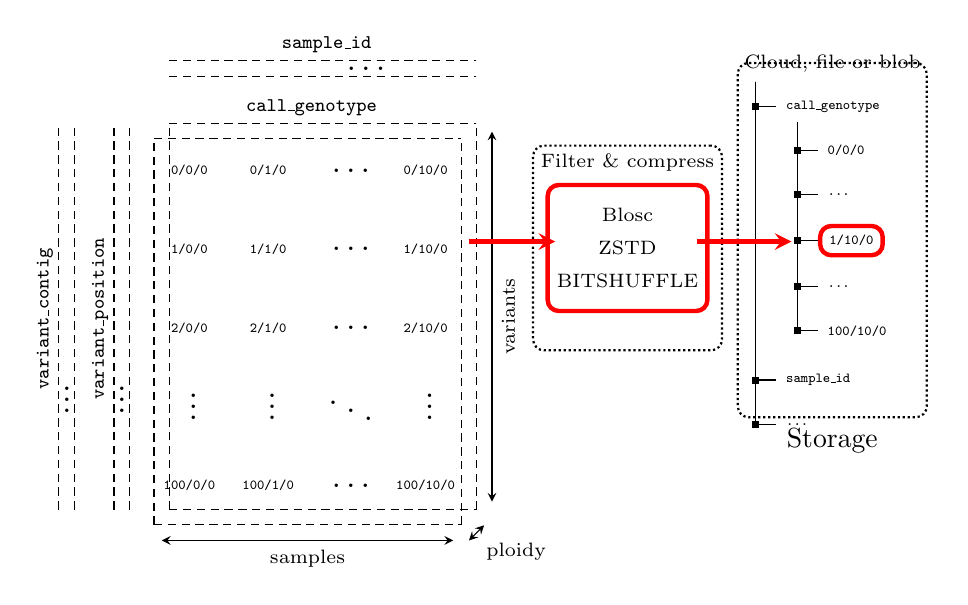
\begin{tikzpicture}


 %% sample_id
  \node at (2.0,5.9,-.5) {\ttfamily \scriptsize sample\textunderscore id};
  % bounds
  \draw[densely dashed] (0,5.5,-.5) -- (3.9,5.5,-.5);
  \draw[densely dashed] (0,5.7,-.5) -- (3.9,5.7,-.5);
 \tikzcuboidset{front face/.style={fill=yellow!20},right face/.style={fill=green!10},top face/.style={fill=yellow!20}}
  \pic at (0,5.5,-.5) {cuboid=.9--.2--0};
  \pic at (1,5.5,-.5) {cuboid=.9--.2--0};
  \node at (2.5,5.6,-.5) {\ttfamily \dots};
  \pic at (3,5.5,-.5) {cuboid=.9--.2--0};

 %% variant_contig
  \node[rotate=90] at (-1.5,2.5,-.3) {\ttfamily \scriptsize variant\textunderscore contig};
  % bounds
  \draw[densely dashed] (-1.4,0,-.5) -- (-1.4,4.9,-.5);
  \draw[densely dashed] (-1.2,0,-.5) -- (-1.2,4.9,-.5);
 \tikzcuboidset{front face/.style={fill=green!10},right face/.style={fill=green!10},top face/.style={fill=yellow!20}}
  \pic at (-1.4,0,-.5) {cuboid=.2--.9--0};
  \node at (-1.3,1.5,-.5) {\ttfamily \vdots};
  \pic at (-1.4,2,-.5) {cuboid=.2--.9--0};
  \pic at (-1.4,3,-.5) {cuboid=.2--.9--0};
  \pic at (-1.4,4,-.5) {cuboid=.2--.9--0};

 %% variant_position
  \node[rotate=90] at (-.8,2.5,-.3) {\ttfamily \scriptsize variant\textunderscore position};
  % bounds
  \draw[densely dashed] (-.7,0,-.5) -- (-.7,4.9,-.5);
  \draw[densely dashed] (-.5,0,-.5) -- (-.5,4.9,-.5);
 \tikzcuboidset{front face/.style={fill=green!10},right face/.style={fill=green!10},top face/.style={fill=yellow!20}}
  \pic at (-.7,0,-.5) {cuboid=.2--.9--0};
  \node at (-.6,1.5,-.5) {\ttfamily \vdots};
  \pic at (-.7,2,-.5) {cuboid=.2--.9--0};
  \pic at (-.7,3,-.5) {cuboid=.2--.9--0};
  \pic at (-.7,4,-.5) {cuboid=.2--.9--0};

 %% call_genotype
  \node at (2.0,5.3) {\ttfamily \scriptsize call\textunderscore genotype};
  % back box
  \draw[densely dashed] (0,0,-0.5) -- (3.9,0,-0.5);
  \draw[densely dashed] (0,0,-0.5) -- (0,4.9,-0.5);
  \draw[densely dashed] (0,4.9,-0.5) -- (3.9,4.9,-0.5);
  \draw[densely dashed] (3.9,0,-0.5) -- (3.9,4.9,-0.5);
 \tikzcuboidset{front face/.style={fill=blue!10},right face/.style={fill=green!10},top face/.style={fill=yellow!20}}
  \pic at (0,0) {cuboid=.9--.9--.5};
  \node at (0.45,0.5) {\ttfamily \tiny 100/0/0};
  \node at (0.5,1.6) {\ttfamily \vdots};
  \pic at (0,2) {cuboid=.9--.9--.5};
  \node at (0.45,2.5) {\ttfamily \tiny 2/0/0};
  \pic at (0,3) {cuboid=.9--.9--.5};
  \node at (0.45,3.5) {\ttfamily \tiny 1/0/0};
  \pic at (0,4) {cuboid=.9--.9--.5};
  \node at (0.45,4.5) {\ttfamily \tiny 0/0/0};
  \pic at (1,0) {cuboid=.9--.9--.5};
  \node at (1.45,0.5) {\ttfamily \tiny 100/1/0};
  \node at (1.5,1.6) {\ttfamily \vdots};
  \pic at (1,2) {cuboid=.9--.9--.5};
  \node at (1.45,2.5) {\ttfamily \tiny 2/1/0};
  \pic at (1,3) {cuboid=.9--.9--.5};
  \node at (1.45,3.5) {\ttfamily \tiny 1/1/0};
  \pic at (1,4) {cuboid=.9--.9--.5};
  \node at (1.45,4.5) {\ttfamily \tiny 0/1/0};
  \node at (2.5,0.5) {\ttfamily \dots};
  \node at (2.5,1.55) {\ttfamily $\ddots$};
  \node at (2.5,2.5) {\ttfamily \dots};
  \node at (2.5,3.5) {\ttfamily \dots};
  \node at (2.5,4.5) {\ttfamily \dots};
  \pic at (3,0) {cuboid=.9--.9--.5};
  \node at (3.45,0.5) {\ttfamily \tiny 100/10/0};
  \node at (3.5,1.6) {\ttfamily \vdots};
  \pic at (3,2) {cuboid=.9--.9--.5};
  \node at (3.45,2.5) {\ttfamily \tiny 2/10/0};
  \pic[ultra thick, red] at (3,3) {cuboid=.9--.9--.5};
  \node at (3.45,3.5) {\ttfamily \tiny 1/10/0};
  \pic at (3,4) {cuboid=.9--.9--.5};
  \node at (3.45,4.5) {\ttfamily \tiny 0/10/0};
  % front box
  \draw[densely dashed] (0,0) -- (3.9,0);
  \draw[densely dashed] (0,0) -- (0,4.9);
  \draw[densely dashed] (0,4.9) -- (3.9,4.9);
  \draw[densely dashed] (3.9,0) -- (3.9,4.9);
  
 %% dimensions
  \draw[stealth-stealth] (0.1,-0.2) -- (3.8,-0.2) node[midway,below] {\scriptsize samples};
  \draw[stealth-stealth] (4,-0.2, 0) -- (4,-0.2,-.5) node[midway,below right] {\scriptsize ploidy};
  \draw[stealth-stealth] (4.1,.1,-.5) -- (4.1,4.8,-.5) node[midway,below,rotate=90] {\scriptsize variants};

%% compresion
 \node (numcodecs) [rectangle, draw, densely dotted, thick, rounded corners, minimum width=2.4cm, minimum height=2.6cm, anchor= south west]
    at (4.8,2.2) {};
 \node[anchor=north,below] at (numcodecs.north) {\scriptsize Filter \& compress};
 %\node[anchor=south,below] at (numcodecs.south) {numcodecs};
 \node (blosk) [rectangle, ultra thick, red, draw, rounded corners, minimum width=1.8cm, minimum height=1.6cm, anchor=center,align=center,text=black]
    at (numcodecs) {\scriptsize Blosc\\\scriptsize ZSTD\\\scriptsize BITSHUFFLE};
 \draw[ultra thick, red,-stealth] (3.9,3.5,-.25) -- (5,3.5,-.25);

%% storage
 \node (location) [rectangle, draw, densely dotted, thick, rounded corners, minimum width=2.4cm, minimum height=4.5cm, anchor= south west]
    at (7.4,1.35) {};
 \node[anchor=south,below] at (location.south) {Storage};
 \node[anchor=center] at (location) {
        \begin{forest}
          for tree={
            font=\tiny ,
            grow'=0,
            child anchor=west,
            parent anchor=south,
            anchor=west,
            calign=first,
            edge path={
              \noexpand\path [draw, \forestoption{edge}]
              (!u.south west) +(7.5pt,0) |- node[fill,inner sep=1.25pt] {} (.child anchor)\forestoption{edge label};
            },
            before typesetting nodes={
              if n=1
                {insert before={[,phantom]}}
                {}
            },
            fit=band,
            before computing xy={l=15pt},
          }
        [{\scriptsize Cloud, file or blob}
          [\ttfamily call\textunderscore genotype
            [\ttfamily 0/0/0]
            [\ttfamily ...]
            [\ttfamily 1/10/0, draw={red,ultra thick, rounded corners}]
            [\ttfamily ...]
            [\ttfamily 100/10/0]
          ]
          [\ttfamily sample\textunderscore id]
          [\ttfamily ...]
        ]
        \end{forest}
 };
 \draw[ultra thick, red, -stealth,rounded corners=5pt] (6.8,3.5,-.25) -- (8,3.5,-.25);
 
\end{tikzpicture} 

}
\caption{Columnar storage of VCF data in chunked, compressed form using Zarr.
[TODO more detail, including brief overview of how data maps from 
VCF to vcfzarr in the examples]
\label{fig-data-model}}
\end{figure}

We propose the \texttt{vcfzarr} specification which maps the 
VCF data model into a columnar layout using the
widely-used Zarr format (Fig~\ref{fig-data-model}). 
Briefly, Zarr is a format 
% FIXME two different uses of $n$ here in a paragraph
for storing $n$-dimensional arrays of a fixed datatype, stored as 
compressed chunks. In the \texttt{vcfzarr} specification, 
each field in a VCF is mapped to an array, which is compressed 
and stored individually allowing for efficient retrieval. 
In particular, call-level data is stored as $m \times n$ arrays
(for $m$ sites and $n$ samples), allowing for efficient 
retrieval of subsets of those fields along both the 
variants and samples axis.
Note that this approach to storing higher dimensional data
sets Zarr apart from more general columnar formats 
such as Parquet [TODO more details and citations?].
See the Methods for more detail on Zarr and the \texttt{vcfzarr}
specification.

\begin{figure}
\begin{center}
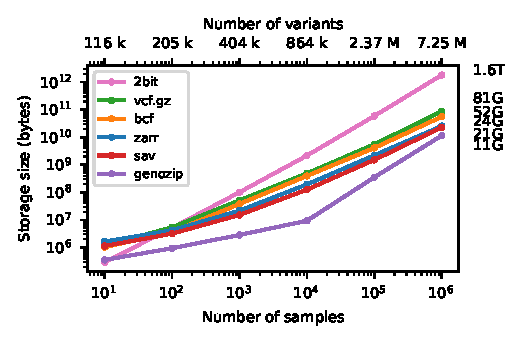
\includegraphics[]{figures/data-scaling}
\end{center}
\caption{Compression performance on simulated genotypes.
Comparison of total stored bytes for VCF data produced 
by subsets of a large simulation of French-Canadians.
Sizes for $10^6$ samples are shown on the right. Sizes 
for Savvy (21.25GiB) and Zarr (22.06GiB) are very similar.
\label{fig-data-storage}}
\end{figure}

Remarkably, the simple approach of compressing
two dimensional chunks with the Zstandard 
compressor~\citep{collet2021rfc} and the bit-shuffle
filter from Blosc~\cite{alted2010modern} produces 
compression levels competitive with specialised methods
on the genotype matrix. In Fig~\ref{fig-data-storage}
we show compression performance on up to a million
samples subset a large and highly realistic 
simulation of French-Canadians~\cite{anderson2023on}
(see Methods for details).
Note that while simulations cannot capture 
all the subtleties of real data, the allele frequency
and population structure patterns in this dataset 
have been shown to closely follow 
observations~\cite{anderson2023on} and so provides 
a reasonable data point when comparing such methods.
% Could note here that this might represent a best 
% case scenario for specialised methods, but maybe 
% not worth bothering with.

[Short note here on why we choose these tools to
benchmark against, and why there's no point in 
a major benchmarkathon. Some recent papers 
have good benchmarks which the interested 
reader can cross-reference]

\subsection{Calculating with the genotype matrix}
Storing genetic variation data compactly is important, but it is also
important that we can analyse the data efficiently. Bioinformatics 
workflows tend to emphasise text files and command line utilities 
that consume and produce text~\citep[e.g.][]{buffalo2015bioinformatics}. 
Thus, many tools that compress VCF data provide a command line 
utility with a query language to restrict the records
examined, perform some pre-specified calculations and finally 
output some text, typically VCF or tab/comma separated values
[TODO check these citations]~\citep{
layer2016efficient, %GQT
li2016bgt, % BGT
tatwawadi2016gtrac, % GTRAC
danek2018gtc, % GTC
lin2020sparse, % SpVCF
lan2020genozip,lan2021genozip, %genozip
lefaive2021sparse, % SAVVY
wertenbroek2022xsi,% XSI
zhang2023gbc}. %GBC
These pre-defined calculations are by necessity limited in scope, however,
and the volumes of text involved in Biobank scale datasets
make the classical approach of custom
analyses via Unix utilities in pipelines prohibitively slow. Thus, 
methods have begun to provide Application Programming Interfaces
(APIs), providing efficient access to genotype and other VCF data
[TODO check these citations]~\cite[e.g.][]{kelleher2013processing,lefaive2021sparse,
wertenbroek2022xsi,zhang2023gbc}. By providing programmatic access,
the data can be retrieved from storage, decoded and then analysed
in the same memory space, avoiding the need for copying
the decoded data and inter-process communication. [TODO some refs
on zero-copy semantics and things like Arrow?]

To demonstrate the accessibility of genotype data and efficiency with 
which calculations can be performed under the different formats,
we use the \texttt{bcftools +af-dist} plugin as an example of such a whole-matrix
computation. 
% The details of the \texttt{af-dist} operation are not important:
% as an example of a whole-matrix operation. 
We chose this particular operation for several
reasons. First, it is a simple but non-trival calculation that requires 
examining every element in the genotype matrix.
Secondly, it produces a small volume of output (a table of
deviations from Hardy-Weinberg expectations in ten allele frequency
bins) and therefore the time spent outputting results is negligible.
Finally, it has an efficient implementation written using the 
\texttt{htslib} C API~\citep{bonfield2021htslib}, distributed as 
a \texttt{bcftools} plugin. 

\begin{figure}
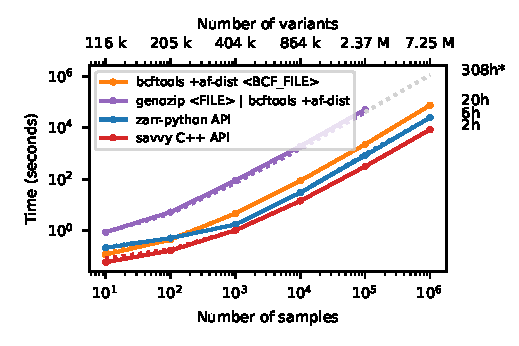
\includegraphics{figures/whole-matrix-compute}
\caption{Whole-matrix compute performance with increasing sample size.
Total CPU time required to run \texttt{bcftools +af-dist}
and equivalent operations in a single thread for various tools.
Elapsed time is also reported (dotted line). Run-time for genozip
at $10^6$ samples was extrapolated by fitting an exponential.
See Methods for full details.
\label{fig-whole-matrix-compute}}
\end{figure}

Figure~\ref{fig-whole-matrix-compute} shows the results of 
running \texttt{bcftools +af-dist} and equivalent operations 
on the data of Figure~\ref{fig-data-storage}. There is a large
difference in the time required (note the log-log scale). 
The slowest approach uses Genozip. Because genozip does not
provide an API and only outputs VCF text, the best approach available 
is to pipe its output into \texttt{bcftools +af-dist}. Thus,
not only must we decode the data from the genozip format, we must 
then parse the large volumes of VCF text and then finally do the 
actual calculation. Running \texttt{bcftools +af-dist} directly
on the gzipped VCF text incurs essentially the same cost, but
the decompression cost is lower and without the interprocess 
communication overhead. Using a BCF file is somewhat faster,
because the packed binary format can be read into the internal 
data structures used by the \texttt{htslib} API more efficiently.

The data shown in Figure~\ref{fig-whole-matrix-compute} for Zarr and Savvy
is based on custom programs written using their respective APIs
to implement the \texttt{af-dist} operation. The Zarr program uses
the Zarr-Python package to iterate over the decoded chunks of the 
genotype matrix and classifies genotypes within a chunk using a 14 line Python
function, accelerated using the Numba JIT compliler~\cite{lam2015numba}.
The allele frequencies and genotype counts are then analysed to produce 
the final counts within the allele frequency bins with 9 lines of 
Python using NumPy~\cite{harris2020array} functions. Remarkably, this 
short and simple Python program is substantially faster than the 
equivalent compiled C using \texttt{htslib} APIs on BCF (6 hours
vs 20 hours for 1 million samples). The fastest method is the 
C++ program written using the Savvy API. This would largely seem
to be due to Savvy's excellent genotype decoding performance
(up to 6.5GiB/s vs 1.2GiB/s for Zarr on this dataset;
Figure~\ref{fig-whole-matrix-decode}). Different choices 
of compressor and filters (zstandard with bit shuffle, in this case) 
would likely lead to improved decoding performance in Zarr,
at the expense of somewhat larger files.

\subsection{Subsetting the genotype matrix}
As datasets grow ever larger, the ability to efficiently access subsets 
of the data becomes more and more important. VCF/BCF achieve efficient 
access to the data for genomic ranges 
by compressing blocks of adjacent records using \texttt{bgzip},
and storing secondary indexes alongside the original 
files with a conventional suffix~\citep{li2011tabix}. 
Thus, for a given range query we 
decompress only the necessary blocks and can quickly access
the required records. 
Methods like Savvy and XSI largely follow the same principles [TODO check and 
be more concrete]. The row-wise nature of these methods, however, mean 
that we cannot efficiently subset \emph{by sample}. In the extreme
case, if we want to access only the genotypes for a single sample
we must still read in and decompress the entire dataset.

\begin{figure}
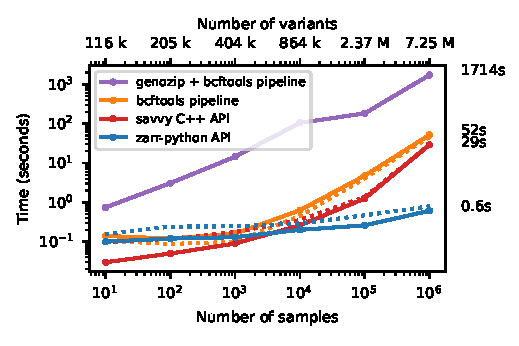
\includegraphics{figures/subset-matrix-compute}
\caption{Compute performance on subsets of the matrix.
Total CPU time required to run the af-dist calculation for
a subset of 10000 variants $\times$ 10 samples from the middle of the matrix
for the data in Figure~\ref{fig-data-storage}.
The \texttt{genozip} and \texttt{bcftools} pipelines involve
multiple commands required to correctly calculate the AF INFO field
required by \texttt{bcftools +af-dist}. See the Methods for full details
on the steps performed.
\label{fig-subset-matrix-compute}}
\end{figure}

We illustrate the cost of row-wise encoding in
Figure~\ref{fig-subset-matrix-compute}, where we run the af-dist calculation
on a small fixed-size subset of the genotype matrices of
Figure~\ref{fig-data-storage}. The two-dimensional chunking of Zarr
means that this small subset of the overall matrix can be efficiently
extracted, and therefore the execution time depends very weakly on 
the overall dataset size, with the overall computation requiring around
1 second for 1 million samples. Because of their 
row-wise encoding for all the other methods CPU time
scales with the number of samples.
Figure~\ref{fig-subset-matrix-compute-supplemental} shows performance
for the same operation when selecting half of the samples in the 
dataset.

\begin{figure}
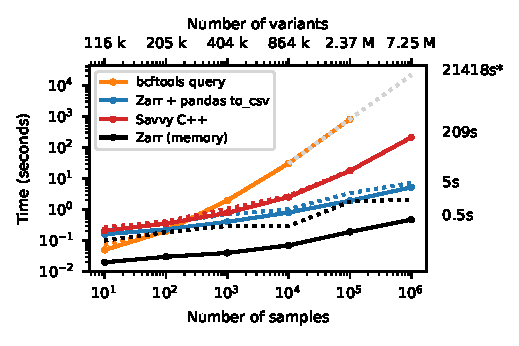
\includegraphics{figures/column-extract}
\caption{Time to extract the genome position and write to a text file.
Total CPU time required to extract the POS field for BCF,
sav and Zar formats
for the data in Figure~\ref{fig-data-storage}.
For the BCF file we used \texttt{bcftools query -f"\%POS$\backslash$n"}.
For sav, we used the Savvy C++ API to extract just the position, 
and output text using the \texttt{std::cout} stream. For Zarr, we read 
\texttt{variant\_position} into a NumPy array, and then wrote to
a text file using the Pandas
\texttt{write\_csv} method. Writing
text dominates in the case of Zarr: populating the NumPy array 
in memory takes less than a second in all cases. Genozip does
not offer an option to extract individual columns, and so would require
the output to be piped into \texttt{bcftools query} or a
Unix utility such as \texttt{cut}.
\label{fig-column-extract}}
\end{figure}

\subsection{Extracting fields}
We have focused on the genotype matrix up to this point, contrasting
Zarr with existing row-wise methods. The genotype matrix, however,
is only one aspect of VCF data.
Real-world VCFs encapsulate much more than just the genotype
matrix, and can contain large numbers of additional fields. Efficient
extraction of the data from these fields is a key use-case
and an area where columnar storage has clear benefits.
Figure~\ref{fig-column-extract} shows the time required to extract 
the genomic position of each variant in the simulated benchmark 
dataset, which we can use as an indicative example of a per-variant 
query. Although Savvy is many times faster than \texttt{bcftools query}
here, the row-wise storage strategy that they share means that 
the entire dataset must be read into memory and 
decompressed to extract just one field from each record. Zarr's
columnar storage excels at these tasks: we only read and decompress
the information required.

\subsection{Case study: Genomics England 100,000 genomes}
In this section we demonstrate the utility of \texttt{vcfzarr} on a large human dataset
and the scalability of the \texttt{vcf2zarr} conversion utility.
Genomics England’s multi-sample VCF dataset (aggV2) is an 
aggregate of 78,195 gVCFs from rare disease and cancer participants 
recruited as part of the 100,000 Genomes Project~\cite{turnbull2018100}. 
The dataset comprises approximately 722 million annotated single-nucleotide 
variants (SNVs) and small indels split into 1,371 roughly equal chunks and 
totalling 165.3 TiB of VCF data after \texttt{bgzip} compression. 
The dataset is used for a variety of research purposes, ranging from 
genome-wide association studies (GWAS)~\cite{kousathanas2022whole} and 
imputation~\cite{shi2023genomics} to 
simple queries involving single gene 
regions~\cite{leggatt2023genotype,lam2023repeat}.

As described in the Methods, conversion to Zarr using 
\texttt{vcf2zarr} is a two-step 
process to limit memory usage and ensure reliability. We 
first converted the 28 VCF files (3.51 TiB) for chromosome 20
into the intermediate columnar format (ICF). This task was 
split into 3899 partitions, and distributed using the Genomics England
HPC cluster. It required about 50 days of CPU, with an elapsed
wall-clock time of about 2 hours. The ICF representation uses a total
of XTiB over XX files and YY directories. We then encoded this intermediate
columnar format to Zarr using 8 cores and XX GB of RAM in about 12 hours.
This produced a dataset with 43 arrays, consuming a 
total of Y GiB of storage over X directories and 
Y files. This is about a 4.8X reduction over the original VCF. 
The top fields in terms 
of storage are detailed in Table~\ref{tab-genomics-england-data}.

\begin{table}
\caption{Summary for a selection of the largest vcfzarr columns produced for 
Genomics England aggV2 VCFs on chromosome 20 using \texttt{vcf2zarr}
default settings. Each field is stored independently 
as a Zarr array with the given type (sufficient to represent all values in the
data). We show the total storage consumed (reported via \texttt{du}) in 
power-of-two units, and the compression ratio achieved on that array.
We also show the percentage of the overall storage that each array consumes.
\label{tab-genomics-england-data}}
\begin{tabular}{llS[table-format=3.1]S[table-format=3.2]S[table-format=3.2]}
\toprule
{Field} & {type} & {storage} & {compress} & {\%total} \\
\midrule
call\_AD &  int16 & 179.7G & 26 & 24.0\\
call\_GQ &  int16 & 171.8G & 13 & 23.0 \\
call\_DP &  int16 & 141.8G & 16 & 18.9 \\
call\_DPF& int16  & 115.1G & 20 & 15.3\\
call\_FT &  string & 58.5G & 160 & 7.8 \\
call\_PL &  int16 & 51.4G & 140 & 6.9 \\
call\_GQX &  int16 & 12.1G & 190 & 1.6 \\
call\_genotype & int8 & 6.1G & 380 & 0.8 \\
call\_genotype\_mask & bool & 3.7G  & 630 & 0.5\\
call\_genotype\_phased & bool & 692.5M  & 1700 & 0.1 \\
call\_PS  & int8  & 102.2M & 12000 & 0.05 \\
variant\_quality & float32 & 22.6M & 2.7 & <0.01 \\
variant\_allele & string & 21.5M & 11 \\
variant\_position & int32 & 12.7M & 4.7 \\
variant\_ABratio & float32 & 9.6M & 6.3 \\
variant\_AN & int32 & 9.6M & 6.3 \\
variant\_filter & bool & 1.9M & 490 \\
\bottomrule
\end{tabular}
\end{table}

% array([23.956     , 22.90533333, 18.90133333, 15.34533333,  7.8       ,
%         6.85333333,  1.61066667,  0.81733333,  0.488     ])

% /call_AD                     int16    179.67 GiB  4.53 TiB       26 125768  37.74 MiB     1.46 MiB            (15912293, 78195, 2)  (10000, 1000, 2)  
% /call_GQ                     int16    171.79 GiB  2.26 TiB       13 125768  18.87 MiB     1.4 MiB             (15912293, 78195)     (10000, 1000) 
% /call_DP                     int16    141.76 GiB  2.26 TiB       16 125768  18.87 MiB     1.15 MiB            (15912293, 78195)     (10000, 1000)
% /call_DPF                    int16    115.09 GiB  2.26 TiB       20 125768  18.87 MiB     959.56 KiB          (15912293, 78195)     (10000, 1000)
% /call_FT                     object   58.5 GiB    9.05 TiB      160 125768  75.48 MiB     487.71 KiB          (15912293, 78195)     (10000, 1000)
% /call_PL                     int16    51.4 GiB    6.79 TiB      140 125768  56.61 MiB     428.51 KiB          (15912293, 78195, 3)  (10000, 1000, 3)
% /call_GQX                    int16    12.08 GiB   2.26 TiB      190 125768  18.87 MiB     100.73 KiB          (15912293, 78195)     (10000, 1000) 
% /call_genotype               int8     6.13 GiB    2.26 TiB      380 125768  18.87 MiB     51.11 KiB           (15912293, 78195, 2)  (10000, 1000, 2)  
% /call_genotype_mask          bool     3.66 GiB    2.26 TiB      630 125768  18.87 MiB     30.53 KiB           (15912293, 78195, 2)  (10000, 1000, 2)  
% /call_genotype_phased        bool     692.51 MiB  1.13 TiB     1700 125768  9.43 MiB      5.64 KiB            (15912293, 78195)     (10000, 1000) 
% /call_PS                     int8     102.2 MiB   1.13 TiB    12000 125768  9.43 MiB      852 bytes           (15912293, 78195)     (10000, 1000) 
% /call_ADR                    int8     102.2 MiB   1.13 TiB    12000 125768  9.43 MiB      852 bytes           (15912293, 78195)     (10000, 1000)
% /call_ADF                    int8     102.2 MiB   1.13 TiB    12000 125768  9.43 MiB      852 bytes           (15912293, 78195)     (10000, 1000)
% /variant_OLD_MULTIALLELIC    object   31.63 MiB   121.4 MiB       3.8 1592  78.09 KiB     20.34 KiB           (15912293,)           (10000,) 
% /variant_quality             float32  22.6 MiB    60.7 MiB        2.7 1592  39.04 KiB     14.53 KiB           (15912293,)           (10000,) 
% /variant_allele              object   21.52 MiB   242.8 MiB      11 1592  156.17 KiB    13.84 KiB           (15912293, 2)         (10000, 2) 
% /variant_position            int32    12.83 MiB   60.7 MiB        4.7 1592  39.04 KiB     8.25 KiB            (15912293,)           (10000,) 
% /variant_ABratio             float32  9.62 MiB    60.7 MiB        6.3 1592  39.04 KiB     6.18 KiB            (15912293,)           (10000,) 
% /variant_AN                  int32    9.6 MiB     60.7 MiB        6.3 1592  39.04 KiB     6.18 KiB            (15912293,)           (10000,) 
% /variant_AC                  int32    9.22 MiB    60.7 MiB        6.6 1592  39.04 KiB     5.93 KiB            (15912293,)           (10000,) 
% /variant_AC_Het              int32    8.98 MiB    60.7 MiB        6.8 1592  39.04 KiB     5.78 KiB            (15912293,)           (10000,) 

% Approx total = 179.67 + 171.79 + 141.76 + 115.09 + 58.5 + 51.4 + 12.08 + 6.13 + 3.66 
% 740, round up to 750
% [179.67 , 171.79 , 141.76 , 115.09 , 58.5 , 51.4 , 12.08 , 6.13 , 3.66 ]
% >>> import numpy as np
% >>> a = np.array([179.67 , 171.79 , 141.76 , 115.09 , 58.5 , 51.4 , 12.08 ,
% 6.13 , 3.66 ]  )
% >>> a
% array([179.67, 171.79, 141.76, 115.09,  58.5 ,  51.4 ,  12.08,   6.13,
%          3.66])
% >>> a / 750 * 100
% array([23.956     , 22.90533333, 18.90133333, 15.34533333,  7.8       ,
%         6.85333333,  1.61066667,  0.81733333,  0.488     ])

Table~\ref{tab-genomics-england-data} shows that the dataset storage
size is dominated by a few columns with the top four
(call\_AD, call\_GQ, call\_DP and call\_DPF) accounting for over 
80\% of the total. These fields are much less compressible
than genotype data (which uses $<1\%$ of the total space here)
because of their inherent noisiness~\citep{lin2020sparse}. By 
default the \texttt{bio2zarr} conversion is lossless, and integers
of the narrowest type required to represent all of the data are
used. In this case, this has resulted in 16 bit integers being used 
for these top four fields. Examining the distribution of the depth
fields, (call\_AD, call\_DP, call\_DPF), we can 
we can see that a tiny fraction of the values stored
are greater than 127 (call\_AD: 0.1\%, call\_DP: xx\%, call\_DPF: x\%; see 
Fig SX for histograms).
One might then reasonably truncate these fields to 8 bit integers.
After converting to 8 bit, call\_AD is reduced by 
x\% (XX GiB) and call\_DP reduced by x\% (XX GiB)
and call\_DPF by x\% (XX GiB). 
Similarly, the vast majority of call\_GQ values (xx\%) are less than 
128 (corresponding to a conditional probability that the genotype call is 
wrong of $10^{-128}$ [TODO CHECK THIS]), and can also reasonably
be truncated. Here, this results in a reduction of x\% (XX GiB).
Combined, truncating these top four fields to 8 bits reduces the 
overall storage of the dataset to XXGiB, corresponding to a 
X-fold compression of the VCF.

% and can reasonably be truncated (a 
% much information would be lost if we used 8 bit
% Substantial
% reductions in space can be achieved, however, if we examine the 
% distributions of these fields and truncate some outliers.
% Figure~SX shows the histogram of the XX call\_AD values, and we can
% see that < 0.0X\% of the values are $>127$. Truncating and 
% re-encoding the call\_AD array as an int8 results in a total storage of 
% XX. A substantial advantage of Zarr is that such per-field optimisations
% can be made after conversion, without affecting the rest of the dataset.
% As discussed in Methods, judicious use of additional filters
% and lossy quantizing can result substantial space savings.

Calculating the histogram of per call values at this 
scale is not a trivial task.
Taking advantage of the rich software ecosystem growing around Zarr
(see Discussion) we used xarray~\citep{hoyer2017xarray}
and Dask~\citep{rocklin2015dask} to transparently distribute the 
computations over a cluster of X workers. 
[ADD DETAILS]
The elapsed time was X minutes, and requires X lines of Python in a 
Jupyter notebook~\citep{kluyver2016jupyter}. 

One of the key uses of the aggV2 dataset is to enable simple queries 
of specific regions. For example, in [A PAPER] they [DID SOMETHING].
We replicated this by running the appropriate bcftools query
on the VCF chunk (note that the user is responsible for finding 
the correct chunk file here, limiting the utility of genomic 
indexes). This took XXX hours.
The same query implemented with the Zarr-python 
API required XXX seconds to produce identical output.

\section{Discussion}

Outline of a possible narrative by paragraph:
\begin{itemize}
\item When VCF was introduced as part of the work of the 1000 Genomes
project the software landscape was a real mess. It has entirely
succeeded in standardising the output of variant callers, and methods
have interoperated well for the past decade. As a method of interchange
following classical file-oriented paradigms it works well enough.
It is also a good archival format: when compressed with a well established
method like gzip and combined with the well-documented description of
the text, we can be sure that files will still be readable decades
from now.


\item VCF is holding back large-scale genomics, however, and in particular the
analysis of population scale genetic variation datasets like UKB and GeL.
Describe the current state of affairs. Variant datasets are chunked up
into reasonable sized bits (10s of gigabytes) so that they can be processed
in parallel. Doing anything with them requires interacting with workflow
managers. In practise, it is not possible to directly write programs to
work across multiple large-scale datasets: although the chunks of data
are given in VCF, orchestrating how the chunks are processed and
the results combined involves substantial work, involving the workflow
manager, and the details of how chromosomes are split into chunks.
Cite examples like the phasing pipelines for UKB from Brownings etc.

\item Distributed computing is the reality, and increasingly datasets
are being mandatorily stored in public clouds as part of
Trusted Research Environments. Cloud object stores are the reality
because it is much cheaper. POSIX file systems are emulated on top of
this. Benefits of breaking up data into manageable pieces are that
compute resources can be localised to the data. Compute resources are
most effectively obtained as short-lived, small VMs that operate
as part of a large cluster. Large vertically scaled ``pet'' servers
are much more expensive, and just not feasible for the current
scale of data. Lots of other architectural
benefits from the new reality of cloud-based storage.

\item Classical methods based around Unix pipelines and streaming
files between processes on a single machine are therefore a
significant mismatch to the reality of large-scale genetic variation
datasets. The majority of methods suggested to make working
with VCF data more efficient are based on these ideas: they all
create a single large file and regard distribution of work
in a cluster as extrinsic. Most output VCF as the result of queries,
which also assumes that the VCF data can be efficiently processed.
This is a reasonable assumption for thousands of samples, but not
for larger datasets.

\item The key issue here is that VCF is not a \emph{computational}
format. Contrast VCF with plink, which stores data on disk in a
form that can be computed on directly. Plink is limited in what
can be descibed though, does not compress, and is not designed
to distributed.

\item The large-scale analysis of genetic variation data does not
need a more efficient file format, which allows files to be downloaded
somewhat more quickly, and subsets extracted somewhat more efficiently
as VCF. It needs a standard storage platform that allows data to be
processed directly without conversion, subsetted efficiently across
both the variant and sample dimensions, with first-class support
for all the necessary additional information (GT values etc),
and that is suited to the realities of today's cloud-based
storage and processing facilities.

\item We suggest that the model used by Zarr is a good choice for this.
We have shown that chunks of the genotype matrix compressed with standard
methods are competitive with highly specialised methods for
genotype data. In reality most of the storage is for non-genotype
data anyway, where everyone is essentially doing the same thing.
Columnar storage allows getting just (e.g.) the variant positions
without reading everything. Another benefit is that by storing
fields separately in different cloud objects, they can have
different permissions. So, users can be given differential access
to read parts of the dataset, and this is managed directly
by the cloud storage. Give example.

\item A major strong point of Zarr is its simplicity. All it's doing
is compressing n-dimensional chunks of numerical data and storing
them using fixed address keys. This key-value approach means that storage
is very flexible and implementation is straightforward. There
are several implementations of the Zarr protocol, and while some of these
are rudimentary, they could be improved or replaced with relatively
little effort. Zarr has been successfully used to store petabytes
of data across different sciences --- genetic variation data is largely
arrays of numerical data, and not really that different ultimately.
Zarr is cloud native.
Zarr is an open specification, built on standard components (contrast
with Hail).

\item Zarr is not perfect. Discuss limitations around ragged arrays,
etc. Forthcoming improvements in zarr v3. The whole genotype matrix
paradigm is challenged by graph genomes as well. While this is
being worked out, there is still plenty of data to analyse as a
genotype matrix.

\item Vision. An ecosystem of tools that interoperate
based on an open, cloud-based format where distribution is naturally
managed by the stored chunks. Tools can be run on different datasets
with minimal tuning, not by writing a full layer of orchestration.
Tools read the data they need, not the entire dataset. Users read
directly from a single canonical dataset, and do not maintain
their own filtered copies. We suggest that the Zarr VCF approach
we have provided would be a good starting point for designing
such a compute platform.

\end{itemize}
[Random fragment to include somewhere]
Row-wise storage of the genotype matrix makes accessing 
sample haplotypes (i.e. the columns),
required for many
applications~\cite[e.g.][]{durbin2014efficient,kelleher2019inferring} 
[TODO add phasing, imputation]
inefficient. The simple approach of storing the genotype matrix
in rectangular chunks allows efficient access both by row \emph{and}
column. Similarly, these rectangular chunks capture patterns
both of similarity between samples and linkage disequilibrium~\cite{mcvean2019linkage} 
between sites, such that conventional compression schemes 
perform very well~\ref{fig-data-storage}.


Reel off Python data science ecosystem: Pandas~\citep{mckinney2010data} etc

\section{Methods}

\subsection{Zarr and block-based compression}
% Zarr is a simple layer on top of best-in-class, modern components
In the interest of completeness it is useful to provide a high-level overview
of Zarr and the techologies that it depends upon. Zarr is a specialised format
for storing large-scale $n$-dimensional numerical data (arrays). Arrays
are split into chunks, which are compressed and stored separately. Chunks are 
addressed by their indexes along the dimensions of the array, and the 
compressed data associated with this key. Chunks are
are often stored in individual files, but a wide array of different
stores are supported including cloud buckets and NoSQL databases. 
Metadata describing the array and its properties is then stored 
in JSON format along with the chunks. Zarr is best seen as a 
\emph{specification} that describes the details of how chunks are 
addressed and stored: there are multiple implementations across
different languages.

Zarr is flexible in allowing different compression codecs and 
pre-compression filters to be specified on a per-array basis.
Two key technologies used by Zarr are the Blosc
% This seems like the best citation for Blosc? It is mentioned here
meta-compressor~\cite{alted2010modern}
and Zstandard compression algorithm~\citep{collet2021rfc}.
Blosc is a high-performance compressor optimised for numerical
data which uses ``blocking''~\citep{alted2010modern} to 
optimise CPU-cache access patterns, as well as highly optimised
bit and byte shuffle filters.  Remarkably, on highly 
compressible datasets, Blosc decompression can be faster 
than \texttt{memcpy}.
Blosc is written in C, with APIs for C, Python, Julia, Rust
and others.

Blosc is a ``meta-compressor'' because it provides different 
access to several different compression codecs. The 
Zstandard compressor~\citep{collet2021rfc} is of particular 
interest here as it achieves very high compression ratios
with fast decompression speeds [see fig]. 
% This may seem a bit off topic, but want to reassure reader that 
% this isn't some niche technology
Zstandard is also used in several recent VCF compression 
methods~\citep[e.g.][]{lefaive2021sparse,wertenbroek2022xsi}.
% LZ4 is also notable - any citations for this?

\subsection{The vcfzarr specification}
The vcfzarr specification is a direct mapping from the VCF data model 
to a columnar binary format, expressed using Zarr. [A HIGH LEVEL 
DESCRIPTION OF THE SPEC, FOCUSING ON RATIONALE BEHIND DECISIONS]

The vcfzarr specification can represent anything described by BCF
(which is somewhat more restrictive than BCF) except for two corner
cases related to the encoding of missing data. Firstly, vcfzarr does
not distinguish between a field that is not present and one that 
is present but contains missing data. [FOR EXAMPLE...]
Because of the use of -1 to represent missing data and -2 to 
represent dimension padding for integers, these values 
cannot be stored. In practise this doesn't seem to be much of 
an issue (we have not found a real VCF that contains negative 
integers). If -1 and -2 need to be stored, a float field
can be used without issues.

\subsection{vcf2zarr}
Converting VCF to Zarr format at Biobank scale is challenging. This main issue is 
around memory usage: although we can view each record in the VCF one-by-one,
we must buffer a full chunk (10,000 variants is reasonable choice) 
in the variants dimension for each of the arrays. 
For VCFs with many FORMAT fields and large numbers of samples this can
easily require tens of gigabytes of RAM per worker, which makes 
parallelism troublesome. Reading the VCF multiple times for different fields
is possible, but would be prohibitively slow for multi-terabyte VCFs.

The \texttt{vcf2zarr} utility solves this problem by first converting 
the VCF data (which can be split across many files) into an Intermediate
Columnar Format (ICF). The \texttt{vcf2zarr explode} command takes a set
of VCFs and stores the data in per-field chunks (by default, 64MiB).
In this way, the memory required is bounded by the size of single record 
BCF record in htslib (plus the size of a decoded bgzf record
[FIXME what is the correct terminology here?]), plus 64MiB for each 
field.  The Intermediate Columnar Format stores the data for each 
field spread across multiple partitions of the data (so that 
multiple parts of the VCF can be read in parallel), and then 
fixed size compressed chunks within those partitions. It also stores information
about the number of records in each partition and chunk of a given
field, so that the record at a particular index can be retrieved efficiently 
later. Summaries such as the minimum and maximum value 
of each field are also maintained, to aid choice of data types later.
A set of VCF files can be converted to intermediate columnar 
format in parallel on a single machine using a given number 
of worker processes using the \texttt{explode} command,
or can be distributed across a cluster using the 
\texttt{dexplode-init},
\texttt{dexplode-partition} and \texttt{dexplode-finalise} commands.

Once the VCF data has converted to the intermediate columnar format,
it can then be converted to Zarr using the \texttt{vcf2zarr encode}
command. Alhough there is a one-to-one mapping between the VCF
fields and the Zarr arrays, there is considerable flexibility 
in how the data is stored, for example in integer width
and compression and filter settings.
By default vcf2zarr chooses integer type sizes based 
on the range of values seen in the intermediate column format
and reasonable compressor defaults, but these can be
altered by generating a schema in JSON format and editing it.
Encoding a given column (for example, \texttt{call\_AD})
involves creating a buffer to hold a full variant-chunk of the 
array in question, and then sequentially filling this buffer with 
values read from the intermediate columnar format. Once the buffer 
is full, the chunks in the samples dimension are compressed
and written to file. [Something about parallelism and distributing]

\section{Choosing default compressor settings}
To inform the choice of compression settings across different fields 
in VCF data, we analysed their effect on compression ratio on 
data from the 1000 Genomes project.

% [FILL IN WITH Shadi's analysis from here:
% https://github.com/sgkit-dev/bio2zarr/discussions/74
% Discussed in:
% https://github.com/sgkit-dev/vcf-zarr-publication/issues/26

\subsection{Benchmarks}
Full details of the benchmarking done in
Figure~\ref{fig-data-storage} and
Figure~\ref{fig-whole-matrix-compute}.
Quick notes:

\begin{itemize}
\item Dataset is based on subsets of French-Canadian sims. We simplify
for increasingly large subsets, keeping only variant sites. We then
convert to VCF and encode to BCF using
\texttt{tskit vcf | bcftools view -O b}.
\item We used a chunk size of XX for sgkit, after some experimentation.
This gave n files of around x MB each for the ``call\_genotypes`` array.
We used the defaults for savvy and genozip.
\item For the afdist CPU time we measure the sum of the total user and
system times required to execute the full command, as reported by GNU
time. Each tool was instructed to use one thread, where the options
were provided. For genozip, the time required to compute
\texttt{genocat file.genozip | bcftools +af-dist}. Because commands
in the pipeline execute concurrently on mutiple cores, the total CPU time is
greater than the elapsed time.
\item Where possible in pipelines we use uncompressed BCF
 output \texttt{-Ou} to make processing more efficient (skip printf
and parsing costs, which are substantial). Following advice
in~\citep{danecek2021twelve}.
\item We do not use BCF output in genozip because it doesn't support
it directly, only VCF (supports BCF by pipeing through bcftools).
\end{itemize}

\section{Availability of source code and requirements}

\section{Data availability}

\section{Declarations}

\subsection{List of abbreviations}
% If abbreviations are used in the text they should be defined in the text at
% first use, and a list of abbreviations should be provided in alphabetical
% order.

VCF: Variant Call Format;

\subsection{Competing Interests}

\subsection{Funding}

\subsection{Author's Contributions}

\section{Acknowledgements}


\bibliography{paper}

\clearpage
\renewcommand\thefigure{S\arabic{figure}}
\setcounter{figure}{0}
\renewcommand\thetable{S\arabic{table}}
\setcounter{table}{0}

\section*{Supplementary Material}

\begin{figure}
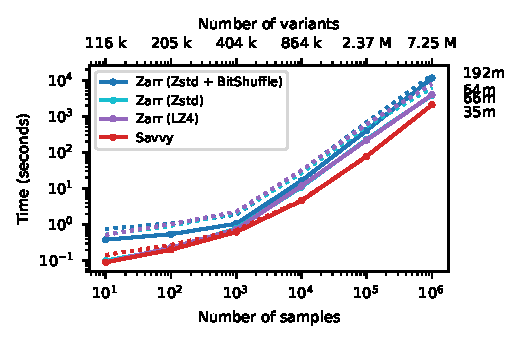
\includegraphics{figures/whole-matrix-decode}
\caption{Genotype decoding performance.
Total CPU time required to decode genotypes into memory using the zarr-python
and Savvy C++ APIs for the data in Figure~\ref{fig-data-storage}.
This corresponds to maximum rate of 1.2GiB/s for Zarr and 5.7GiB/s
for Savvy. [TODO add data for 1 million samples]
\label{fig-whole-matrix-decode}}
\end{figure}

\begin{figure}
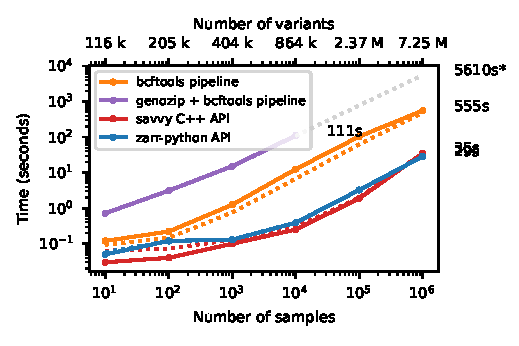
\includegraphics{figures/subset-matrix-compute-supplemental}
\caption{Compute performance on a large subset of the genotype matrix.
Total CPU time required to run the af-dist calculation for
a subset of half of the samples and 10000 variants from the middle of the matrix
for the data in Figure~\ref{fig-data-storage}.
Genozip did not run for
$n > 10^4$ samples because it does not support a file to specify
sample IDs, and the command line was therefore too long for the shell
to execute. 
\label{fig-subset-matrix-compute-supplemental}}
\end{figure}


\clearpage
\section*{Text graveyard}

Here's a bunch of text that contains bits that might be useful and readapted.


\subsection{Chunked storage and distributed computation}
How we store genetic data fundamentally affects how computation
can be structured, and ultimately the scalability of the calculations
we wish to perform. Classically, genetic variation data is stored via one
of two strategies. The first strategy, epitomised by
VCF~\citep{danecek2011variant} encodes all the data for a given
variant in a record, and then stores these records consecutively on file
(optionally compressed). This record-oriented approach maps well to the
powerful Unix pipelines abstraction and
has proven to be very successful.
The second classical strategy, epitomised
by the \texttt{plink} BED format~\citep{purcell2007plink}, is to
store genotype data in a structured binary format that can be
accessed directly. This memory-map approach tends to
be much faster to access, but leads to larger files and is more
limited in what can be represented. There are advantages and
disadvantages to both approaches, but one problem fundamentally
limits their utility for modern datasets: neither is well suited to
scaling-out across multiple machines.

[Probably need a paragraph here on what we've done classically
by splitting by variant. This was the dominant dimension, so that
worked fine. Now we need to also think about access-by-sample]

Given the scale of modern datasets, the ability to perform
calculations in parallel on multiple CPU cores
is now a basic prerequisite, and
running concurrently on multiple computers in a cluster
is increasingly becoming necessary. [For interactive analysis? People have
been doing concurrent computing with HPC clusters forever.]
Record-oriented variant storage such as VCF is not suitable
for  distributed computing because although it is relatively
straightforward to break workloads up by variant, we cannot efficiently
split by sample (see the section on Columnar Data below for details).
Storing data in a memory-mapped manner, where the genotypes
for each variant are written consecutive consecutively to a file,
suffers from the same problem. Although it is useful to conceptualise
the genotype matrix as two-dimensional, it is important to remember
that computer memory and file storage is ultimately one-dimensonal.
For example, plink's memory-mapped data layout linearises the 2D
genotype matrix by writing [TODO check] $n$ bytes representing
the genotypes for all samples at a variant position consecutively.
Because the genotypes for a given variant index can be found
in contiguous blocks at easily computable offsets from
this initial location in memory,
accessing the genotypes for a given variant is very efficient.
However, accessing the genotypes for a given sample at every
variant position is much less efficient because each of the $m$ bytes we
must read are $n$ bytes apart in the file.
In the distributed context, this often means
that each compute node  in a
cluster must effectively read the entire file in order to obtain the
data for a subset of samples. In practise, this means that calculations
are limited by I/0 bandwidth.


A simple and elegant solution to providing efficient access to such
large matrices across multiple dimensions is to store rectangular
\emph{chunks} rather than entire rows or columns. This is illustrated
in Fig~\ref{fig-data-storage}, where we show the basic approach
used by sgkit. By storing data in these regular chunks, we
can efficiently access data for both specific variants \emph{and}
samples.

Additionally, we can compress the individual chunks [more details].

This general strategy for storing multidimensional numerical data
has been in use for many years~\citep{folk2011overview}

This maps well to distributed computing because Zarr provides a
very flexible approach to storing the chunks. By using a native cloud store
for these chunks, compute nodes can directly access the chunks that
are needed, and not read irrelevant data.
[TODO flesh out and more stuff.]


\subsubsection{Array oriented computing}

NumPy~\citep{harris2020array} has been transformational, and provides
the basic framework for scientific computing in Python.

[ Things to cite: pandas~\citep{mckinney2010data},
BioNumpy~\citep{rand2022bionumpy}, OME-Zarr~\citep{moore2023ome}]

[NOTE: we may also want a section discussing the n-dimensional array model,
but I think this section is the right place to discuss that?]

\subsubsection{Columnar binary data}

Perhaps the most important factor limiting scalability in contemporary genomics
is the continued reliance on row-wise storage of data---most often
encoded as blockwise-compressed text.
[Explain why row-wise is bad without reference to specific genomics applications.]

The Variant Call Format (VCF) is the standard method for interchanging
genomics data~\citep{danecek2011variant}.
In VCF each row describes the observations for a set of samples
at a given position along the genome, and consists of fixed columns such as the
genome position as well as per-sample columns. [More info]
VCF was introduced as part of the 1000 Genomes project, and works reasonably
well at the scale of 1000s of samples. However, when we have hundreds of
thousands of samples it becomes extremely unwieldy
. For example, the
phased genotypes for 200K samples in UK Biobank produced by Browning [cite]
require X GB of space.
(Note that this file contains no extra INFO keys; in practice a great deal
more information is stored in the VCF leading to files that are orders of
magnitude larger, and requiring them to be split into chunks, further
increasing their unwieldiness.)
Running [a simple query that requires only looking at
one column] on this file like X required Y minutes.

[TODO be more concrete here; what is the thing we're summarising?]
This slow response time to a simple query is primarily caused by the row-wise
nature of VCF (and BCF), because in order to read a single piece of
information about a particular variant site we must read \emph{all}
the information
about that site. Then, if we wish to summarise that information over
all sites, then we must read the entire dataset.

A lesser but still significant cause of inefficiency is the use of
text to store the data. [More info]

These issues are of course well known, and there are numerous projects
that seek to alleviate them. [Discuss] They're all quite bespoke to genomics data
through.

In sgkit we use Zarr which although initially introduced to store
genomics data, has now been adopted widely in [X, Y and Z].
Zarr is [description] and has [advantages]

Also to discuss (not sure how these fit in to this specific sectio
on background technologies vs existing genomics infrastructure; can
sort out later):

\begin{itemize}
\item columnar (with small records) good for I/O elimination + sequential access.
Classical locality of reference stuff as well.
\item What does this mean with ND arrays? Slippery concept. Discuss.
\item Compression improvements from columnar.
\item Poor performance of text-based VCF has been noted many times,
and lots of prior work in this space e.g. \citep{kelleher2013processing}
\item Honourable mentions for bcftools~\citep{danecek2021twelve},
htslib~\citep{bonfield2021htslib}, CRAM~\citep{bonfield2014scramble,bonfield2022cram}
which uses a columnar approach
\end{itemize}


\subsection{Storing genetic variation data}

It is important to note that the example in Fig.~\ref{fig-data-storage}
is something of a best-base
scenario in terms genomic dataset storage, in that we are only
storing genotype data (per sample, per variant),
and, because it is error-free, is very
highly compressible. Noisier genotypes will not compress quite
so well, and storing less compressible data (such as genotype
quality values) results in a large increase in the overall
storage size. This is essentially unavoidable, but the Zarr-based
approach still has some significant advantages over VCF/BCF
[basically we can store separately and come up with distinct
compression strategies based on the data type. Dunno if we
want to get into this here. This is a complex topic with
a lot of existing work which we should review and reference,
and this is maybe not the place to do it.].

[SpVCF has some good text on high-entropy QC measures. We have to
reduce this entropy or we just can't store the data]


[Why are we reviewing all this? Well, we want to make the point
that people have been trying hard to address the problem of
how to deal with large-scale genomic data for quite a while,
and have come up with lots of specialised methods. There
are a few things to keep in mind. Our approach is to use
standard methods just on the "rectangles" of variant data
and it's already quite good. You could imagine writing specialised
compression filters for genotypes, if you wanted (maybe a
discussion item though). The key thing is the \emph{interface}.
They're all tying to the command line and to classical
sequential workflows. We have Python, and distributed compute. ]

Storage is the foundation on which any large-scale data-driven computation
rests: how we encode and organise data on persistent storage (the format)
fundamentally affects and limits the efficiencies of downstream calculations.
Different formats are optimised for different purposes, and there are
often many competing requirements when designing a data storage format.
% TODO is there some literature we could cite on this? I'm making up the
% term "computational format" here, presumably there is lots  prior thought
% on these ideas?
For our  purposes here, it is important to distinguish between \emph{archival}
and \emph{computational} formats. An archival format is optimised for
maximum interoperability and future-proofing, and uses the simplest and
most robust technologies to ensure the long-term usability of the data.
Reasonable compression levels are important because
of storage and transfer costs, but the efficiency of data access is a
secondary concern.
A computational format, on the other hand, is optimised
for calculations, for \emph{using} the data, today. A computational format
is designed with particular data access patterns in mind, ultimately
to make a broad range of queries and downstream computations as efficient as
possible.

% Note: a quick explanation of VCF for CS people coming in fresh
VCF~\citep{danecek2011variant} is a text-based format in which each line
describes observations
and metadata for a single variant (a position on the genome at which
variation occurs in the sample). The first eight tab-delimited
columns are mandatory, and subsequent columns describe the per-sample
genotype calls and quality control data.

[WIP: currently working on weaving together the stuff below into
some sort of narrative]


SeqArray~\citep{zheng2017seqarray} and the GDS format~\citep{zheng2012high}
provide efficient storage and programmatic access in R.


The approach taken by \toolname{plink}~\citep{purcell2007plink,chang2015second} is to
store data in an uncompressed binary format. This has some major
advantages.

BGEN \citep{band2018bgen} is optimised for storing large-scale
genotype array data and stores probabilities, and is used
in particular by UK Biobank~\citep{bycroft2018genome}
[Should consider the "hard-call" nature of most of these formats]

Many methods working with large scale genetic
data now use the PBWT or variants of
it~\citep[e.g.][]{li2016bgt,lefaive2021sparse,wertenbroek2022xsi}. PBWTs have
disadvantages, however: data must be phased, and compression level
is quite sensitive to the presence of errors [citation? people have
worked around this]

Several tools provide querying interfaces in their CLIs
(reminiscent of SQL) to provide easy access to particular samples, or
variants~\cite{li2016bgt,layer2016efficient}.

More recently XSI~\citep{wertenbroek2022xsi} is an file format that
uses a combination of strategies to achieve excellent compression
performance, and can support some calculations directly on the
compressed format. It provides a command line interface and a
C API.

The SAV format is an extension of BCF that takes advantage
of the sparseness of large scale genomic datasets~\citep{lefaive2021sparse}.
They provide a command line interface and a C++ API.
% TEXT from HSG chapter section on compressing data

% The simplest approach to compressing such data is to organise it in a
% `variant-centric' fashion, such that all observed genotypes for a given variant
% are stored in a contiguous block. Because most variants are rare, this will
% result in long runs of identical values that compress well using standard
% methods. This is the approach taken by the Variant Call
% Format~\citep{danecek2011variant}, and its more efficient binary encoding, BCF.
% The compression levels achieved by this straightforward approach are good, and
% quite competitive with more sophisticated methods. The disadvantage
% is that many queries require full decompression of the data, which can be
% prohibitively time-consuming. The SpeedGene data format and software
% library~\citep{qiao2012handling} chooses from one of three encoding methods for
% each SNP determined by the allele frequency; \cite{sambo2014compression} extend
% this idea by identifying blocks of SNPs in LD, and adding two additional
% potential encodings utilising this information.

% An alternative to this variant-centric approach is to store genotypes in a
% `sample-centric' fashion. Here, all genotypes for a particular sample are
% stored consecutively. While this breaks the simple repetition structure of data
% stored in variant-centric form, other methods can be employed to find
% compressible structure. For example, TGC~\citep{deorowicz2013genome} compresses
% sample genotypes using a custom Lempel-Ziv style approach on runs of identity
% among samples. This explicit use of LD structure results in excellent
% compression performance (for example, 32MB for all SNPs in 1000 Genomes
% chromosome 1); unfortunately, querying a dataset requires full decompression,
% making the format unsuitable for online analysis. The GQT
% toolkit~\citep{layer2016efficient} also uses the sample-centric organisation of
% genotype data, but takes a different approach to compression. Variants are
% sorted by allele frequency (resulting in longer runs of identical values within
% samples) and then compressed using an efficient bit-vector
% representation~\citep{wu2002compressing}. The resulting file-sizes are similar to
% compressed BCF, but many queries can be performed directly on the compressed
% representation and are therefore many times faster.

% The positional Burrows-Wheeler transform~\citep{durbin2014efficient}, or PBWT,
% is another sample-centric method. Building on the success of Burrows-Wheeler
% transform applications in
% genomics~\citep{langmead2009ultrafast,li2009fast,li2009soap2}, PBWT provides
% very good compression performance and efficient algorithms for finding
% haplotype matches. The algorithm builds a representation of the data based
% on sorted haplotype prefixes in linear time, and the LD structure of the data
% ensures that the sorting orders between adjacent sites change very little
% on average. The method has been successfully applied
% to phasing~\citep{loh2016reference}, detection of IBD
% segments~\citep{naseri2017ultra}, improving the performance of the Li and
% Stephens model~\citep{lunter2016fast}, and a general query engine for genotype
% data~\citep{li2016bgt}. Recent extensions include privacy preserving
% search~\citep{shimizu2016efficient} and generalisation to the setting of graph
% genomes~\citep{novak2017graph}.


\subsection{Distributed computation}
Distributed computation has been the reality in the analysis
of genetic variation for many years,
where data is most often provided as per-chromosome VCFs.
This chunking provides a fairly straightforward way to parallelise
computations, using HPC schedulers to split work per-file.
When more fine-grained parallelism is required, users must
provide exact genome coordinates of the genome regions
as part of their submission scripts. Combining results
is a manual operation.
Workflow engines such as
Snakemake~\cite{koster2012snakemake,molder2021sustainable}
and [TODO mention WDL, Cromwell, etc?] make such analyses
much easier, but there is still a great deal of room for
mistakes.
Per-chromosome VCFs are not practical for biobank scale
projects, however, and variant call data tends to be split
into many (still large) files.
For example, the VCFs for 150K UKB WGS data~\cite{halldorsson2022sequences}
are provided in 50kb chunks~\cite{browning2023statistical}, resulting in
hundreds of files per chromosome.
% This is horrible writing, but the point is important.
While these files provide a natural
unit for distributing work, the details of how they
are split differ and essentially there is
no interoperability among large-scale datasets because the VCFs are
so cumbersome that a separate orchestration layer is required to
access the data in parallel.

Despite this long history of de-facto distributed computation
and the clear need for better methods of accessing genetic
variation data in a distributed fashion, there is almost
no scientific literature on the topic (in stark contrast to the
study of methods to compress a VCF into a single file,
as discussed in section XXX).

[This is a really rough outline, also not sure how exactly
we sequence the ideas here. Just getting paragraph fragments
on paper. We do need to explain something of the hadoop ecosystem
to readers who are not familiar, though.]
Distributed analytics for large-scale data is a mature
techology, with many different approaches. Hadoop~\citep{white2012hadoop}
is the original method, and remains the basis of the
dominant ecosystem. HDFS. Spark [CITATION?] lets us
do more complex analytics. Parquet [CITATION?]

Although the Hadoop ecosystem has been hugely successful
in many domains, it has had a limited impact in genomics.
[List some things that have been tried for e.g variant calling
, like ADAM~\citep{nothaft2015rethinking}].
[Briefly mention two approaches using Hadoop clusters
~\citep{boufea2017managing,fan2020variant}, to not very
exiting results].

[Hadoop/Spark/Parquet are fundamentally unsuited to genetic
variation data [WHY]?]

Discuss Hail. It's awesome, has enabled current
generation of mega-scale projects. Drawbacks are the
architecture has emphasised performance etc over adaptability
and simplicity. Uses bits of Spark for X, but custom YZ .
File format is undocumented, etc.

Discuss why the sgkit architecture is suited to distributed
computation. Discuss Zarr's use in cloud stores, and existing
deployments. Discuss Dask.
We do not attempt a head-to-head performance comparison with
Hail here, but defer to Liangde's thesis~\citep{li2022efficient}
with brief summary.
Forward ref to following sections on applications to demonstate
sgkit in a distributed context.


\end{document}

